\section{Langkah-Langkah Percobaan}

\begin{enumerate}
    \item Sambungan LAN dilakukan dari laptop ke router, kemudian dari router ke router
    \item Login lewat MAC address, dilanjutkan dengan reset router via Winbox
    \begin{figure}[H]
        \centering
        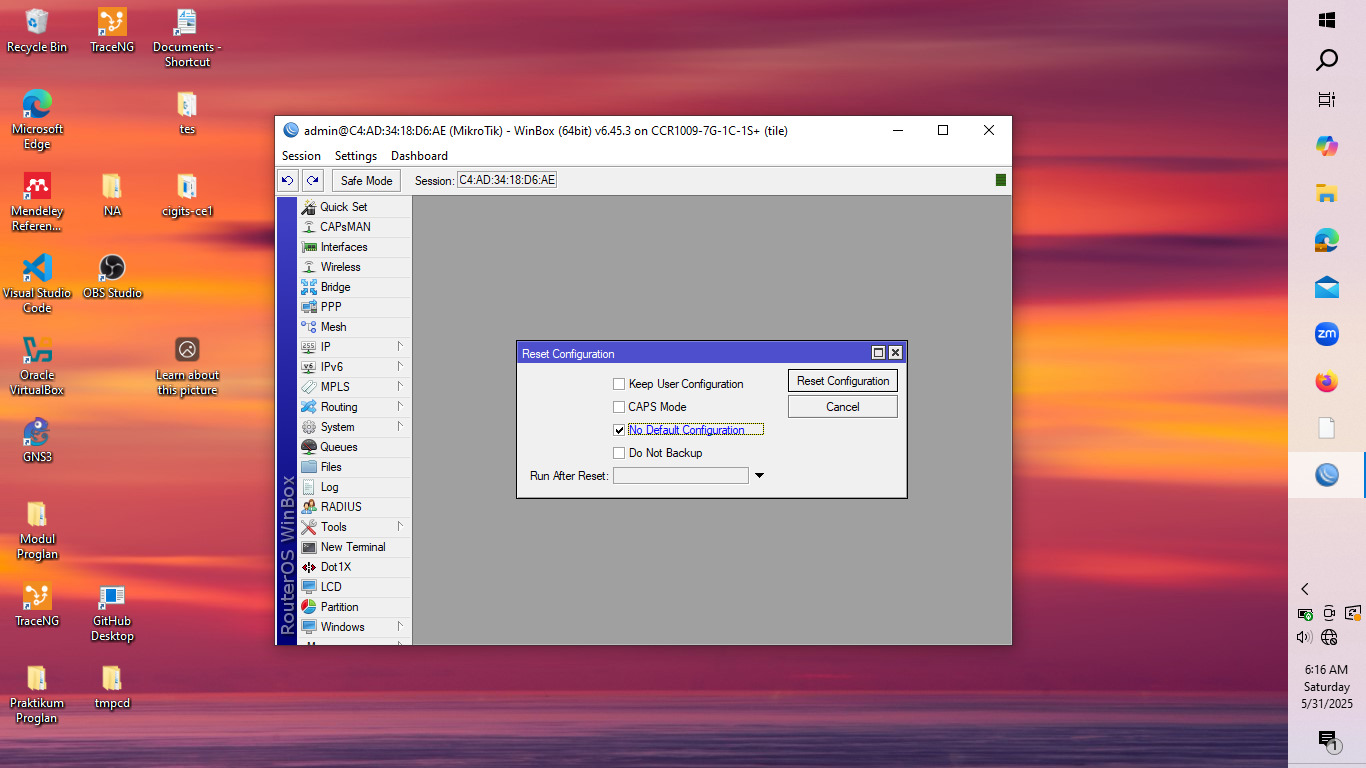
\includegraphics[width=0.5\linewidth]{P1/img/gambar1.jpeg}
        \caption{Reset konfigurasi router lewat Winbox}
        \label{fig:reset-router}
    \end{figure}

    \item Konfigurasi DHCP dilakukan
    \begin{figure}[H]
        \centering
        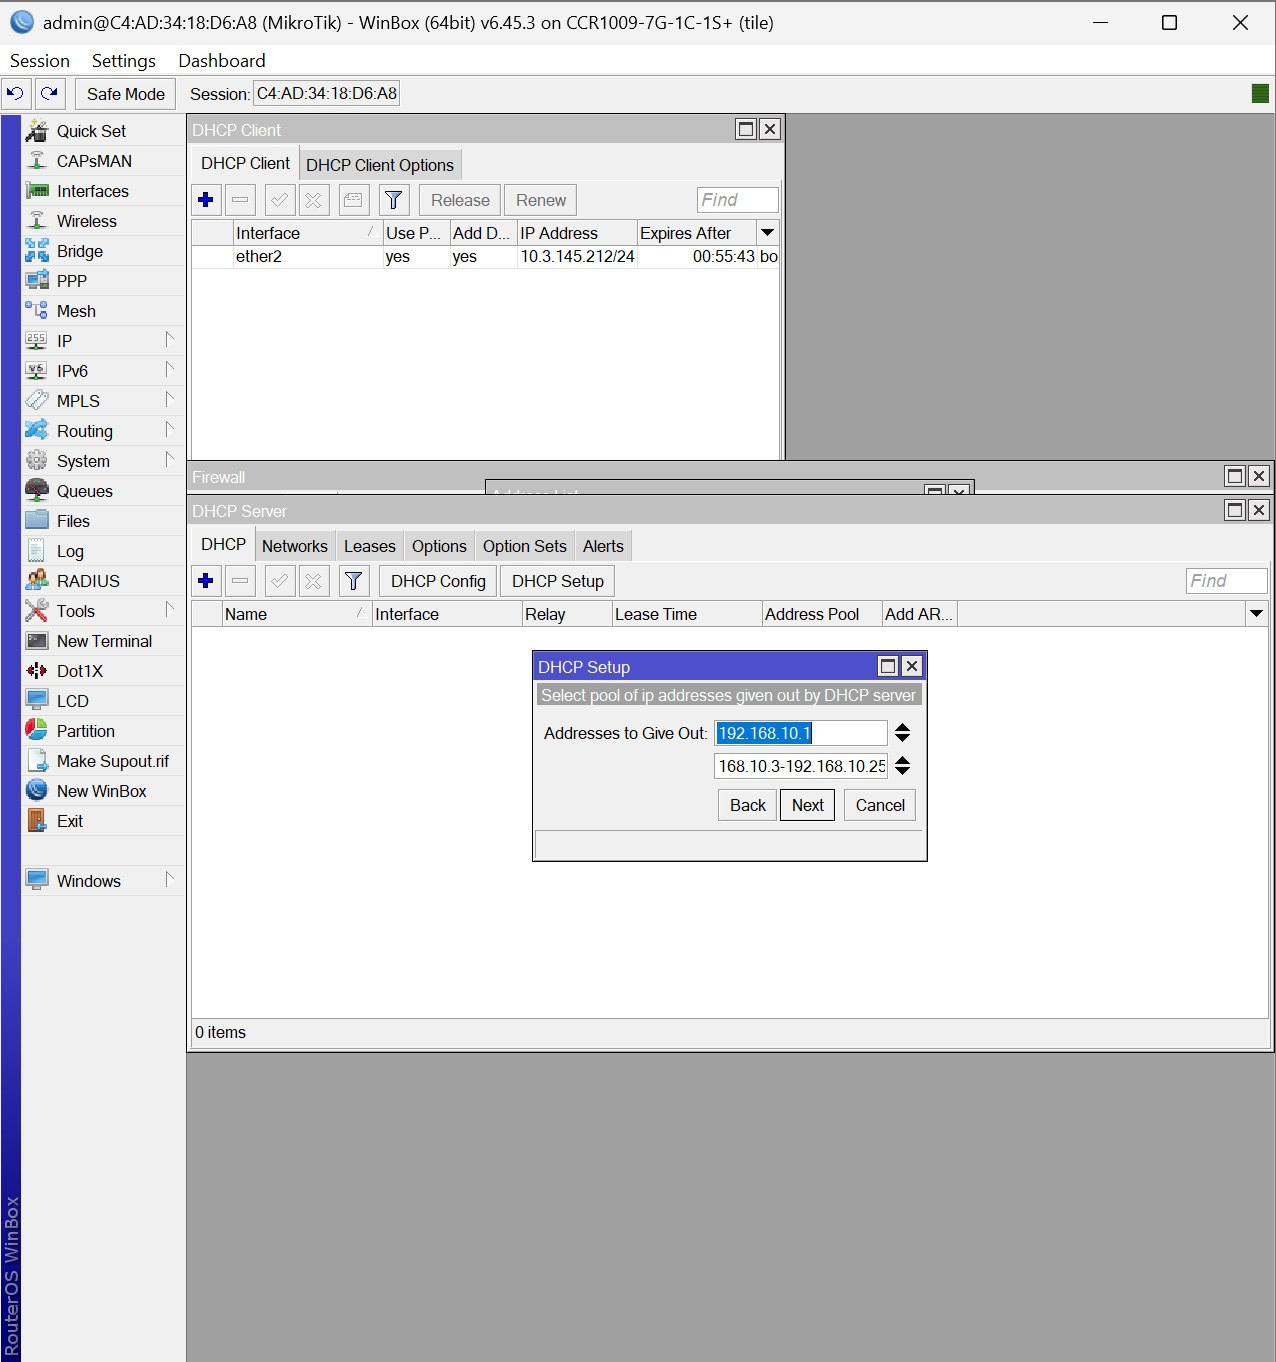
\includegraphics[width=0.5\linewidth]{P1/img/gambar2.jpeg}
        \caption{Konfigurasi DHCP Client dilakukan pada router dengan koneksi internet}
        \label{fig:DHCP-router-A}
    \end{figure}
    
    \item Firewall dengan fitur NAT dikonfigurasi
    \begin{figure}[H]
        \centering
        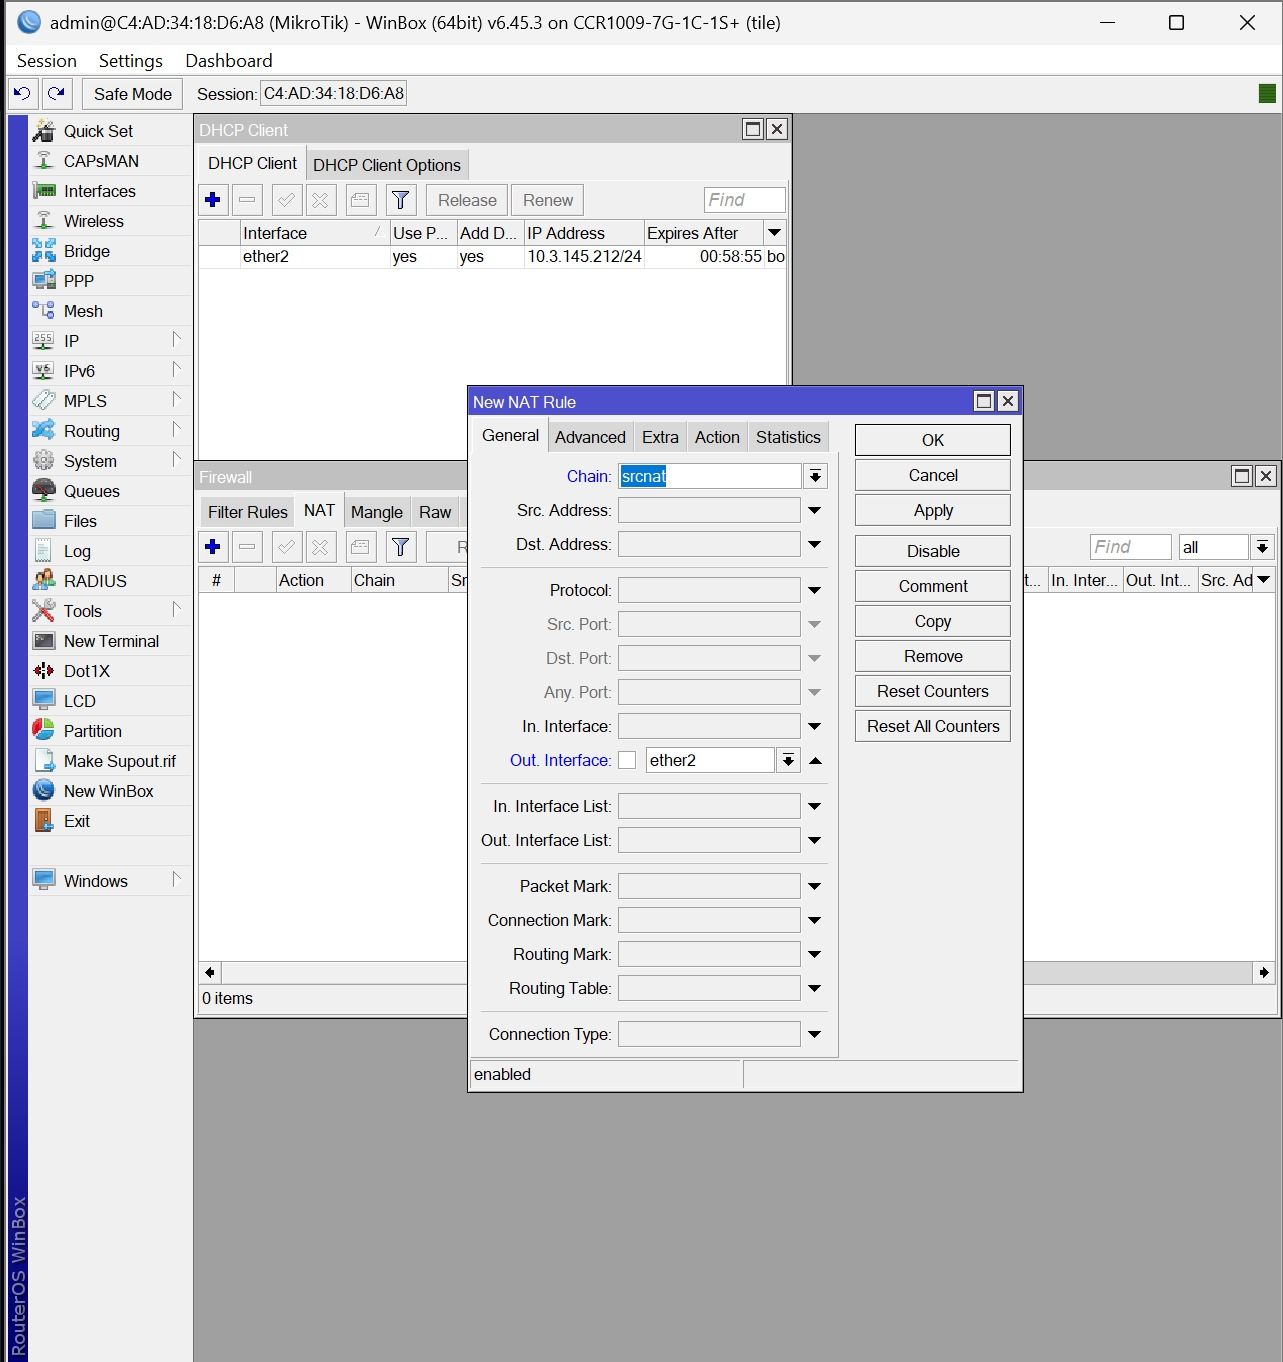
\includegraphics[width=0.5\linewidth]{P1/img/gambar3.jpeg}
        \caption{Mengonfigurasi IP di ether3}
        \label{fig:Firewall-NAT}
    \end{figure}
    
    \item Konfigurasi IP dilakukan pada jaringan lokal melalui ether1.
    \begin{figure}[H]
        \centering
        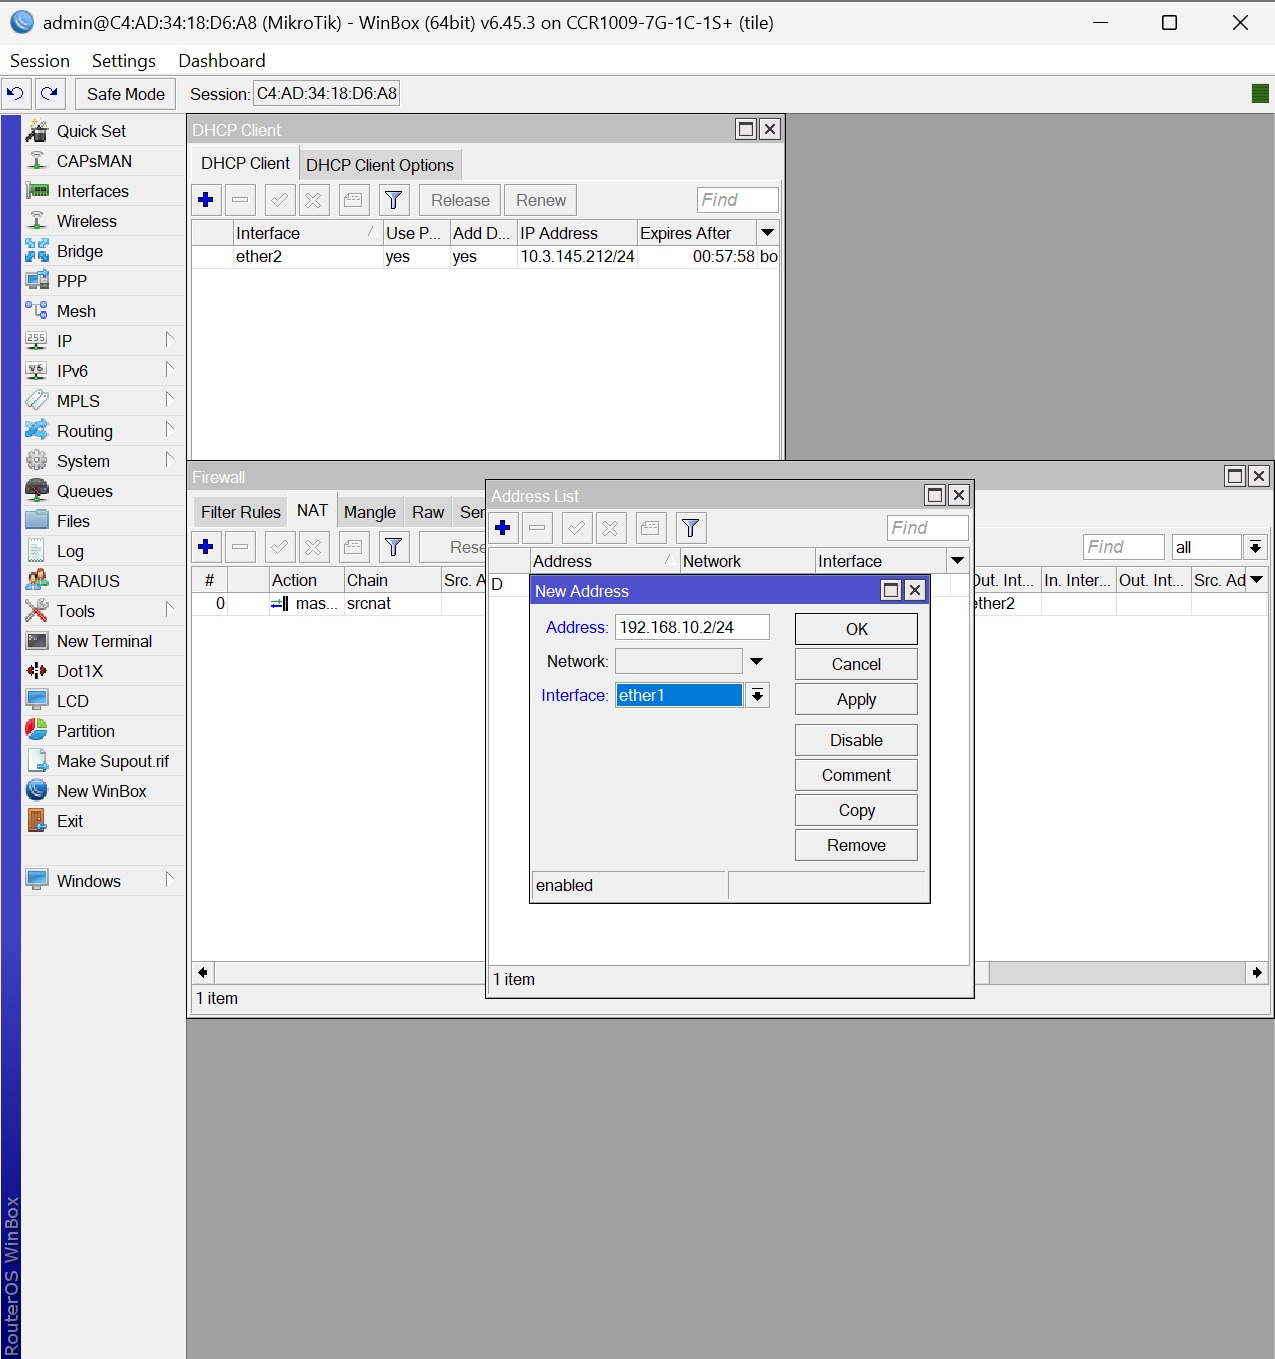
\includegraphics[width=0.5\linewidth]{P1/img/gambar4.jpeg}
        \caption{Konfigurasi DHCP server dilakukan pada Mikrotik}
        \label{fig:Alamat-IP-ether}
    \end{figure}
    
    \item DHCP server dikonfigurasi guna memberikan IP kepada klien
    \begin{figure}[H]
        \centering
        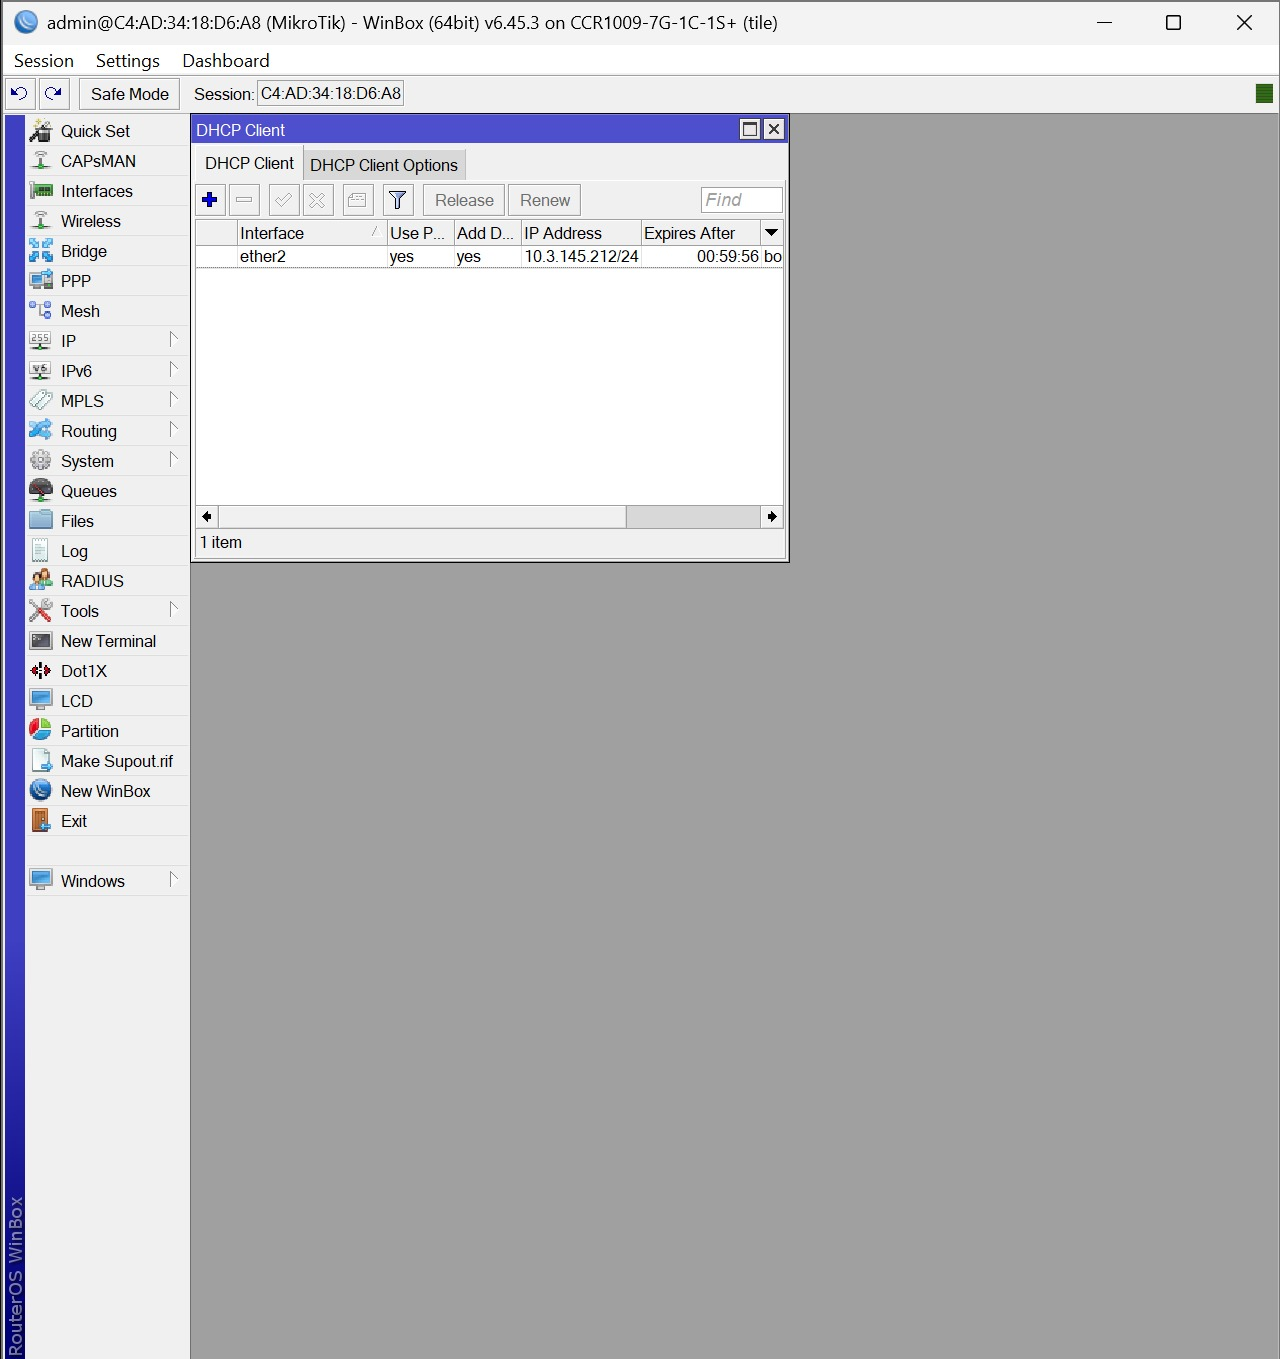
\includegraphics[width=0.5\linewidth]{P1/img/gambar5.jpeg}
        \caption{Konfigurasi DHCP server dilakukan di Mikrotik}
        \label{fig:DHCP-server-mikrotik}
    \end{figure}
    
    \item Aktivasi Proxy ARP dilakukan
    \begin{figure}[H]
        \centering
        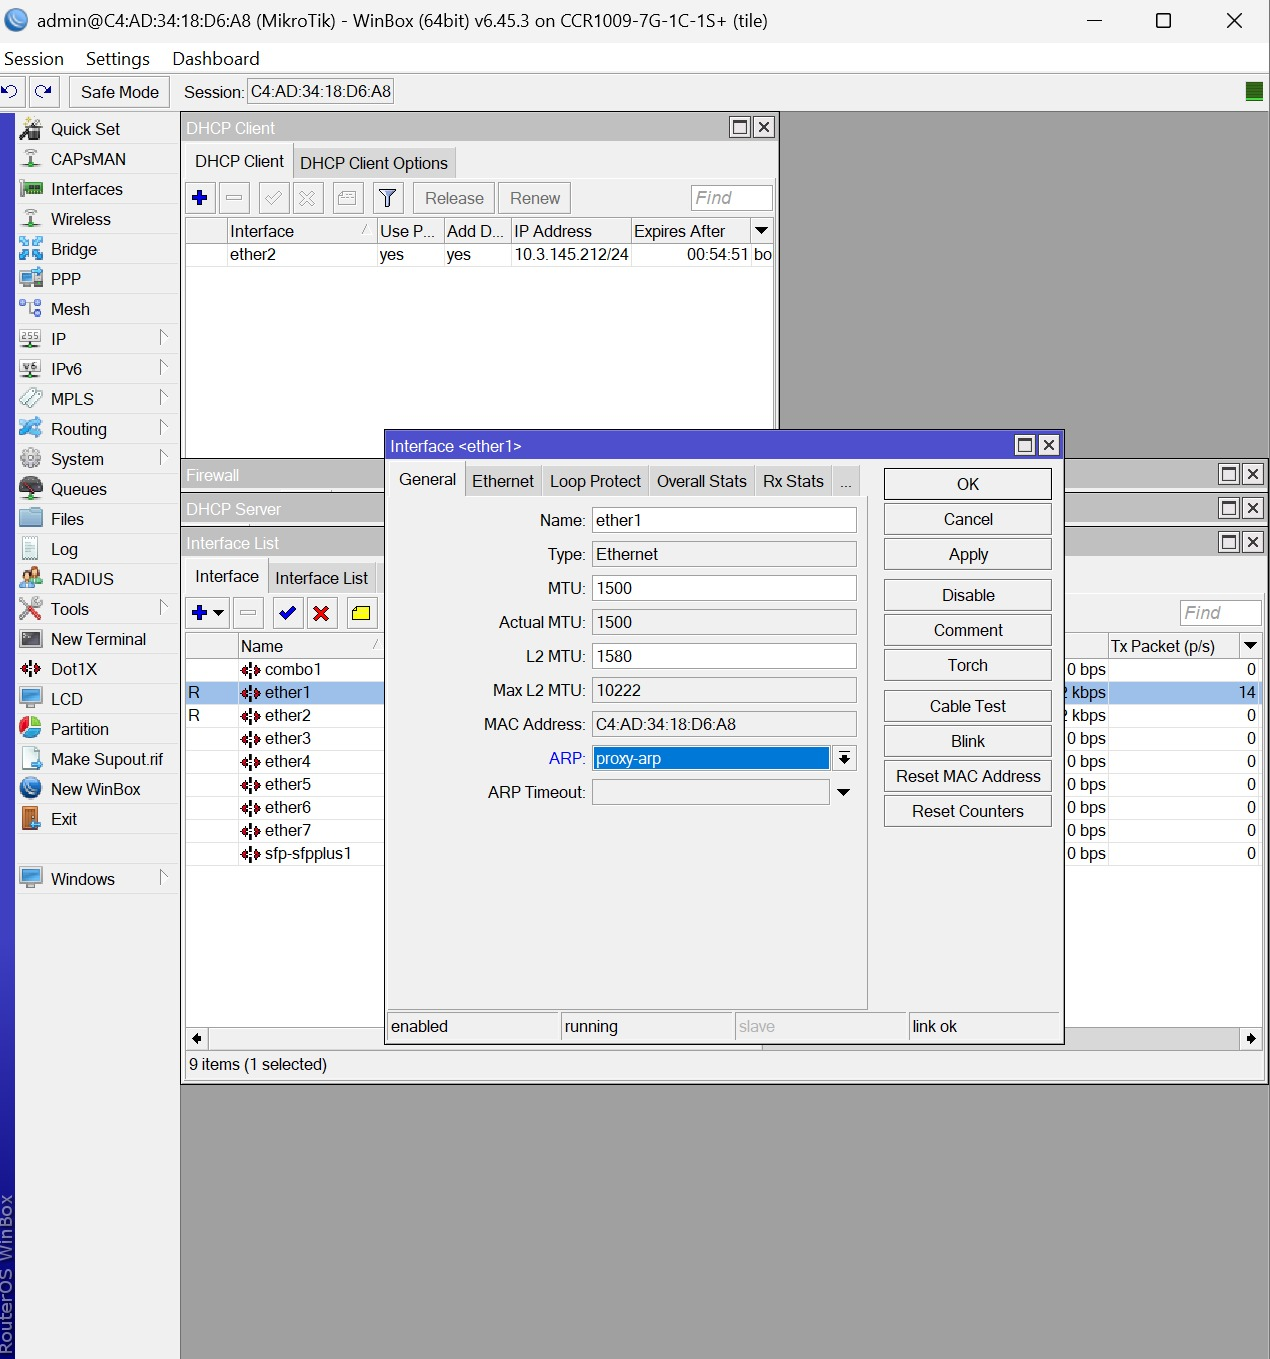
\includegraphics[width=0.5\linewidth]{P1/img/gambar6.jpeg}
        \caption{Aktivasi fitur Proxy ARP}
        \label{fig:Proxy-ARP}
    \end{figure}
    
    \item Mengonfigurasi server untuk koneksi PPTP
    \begin{figure}[H]
        \centering
        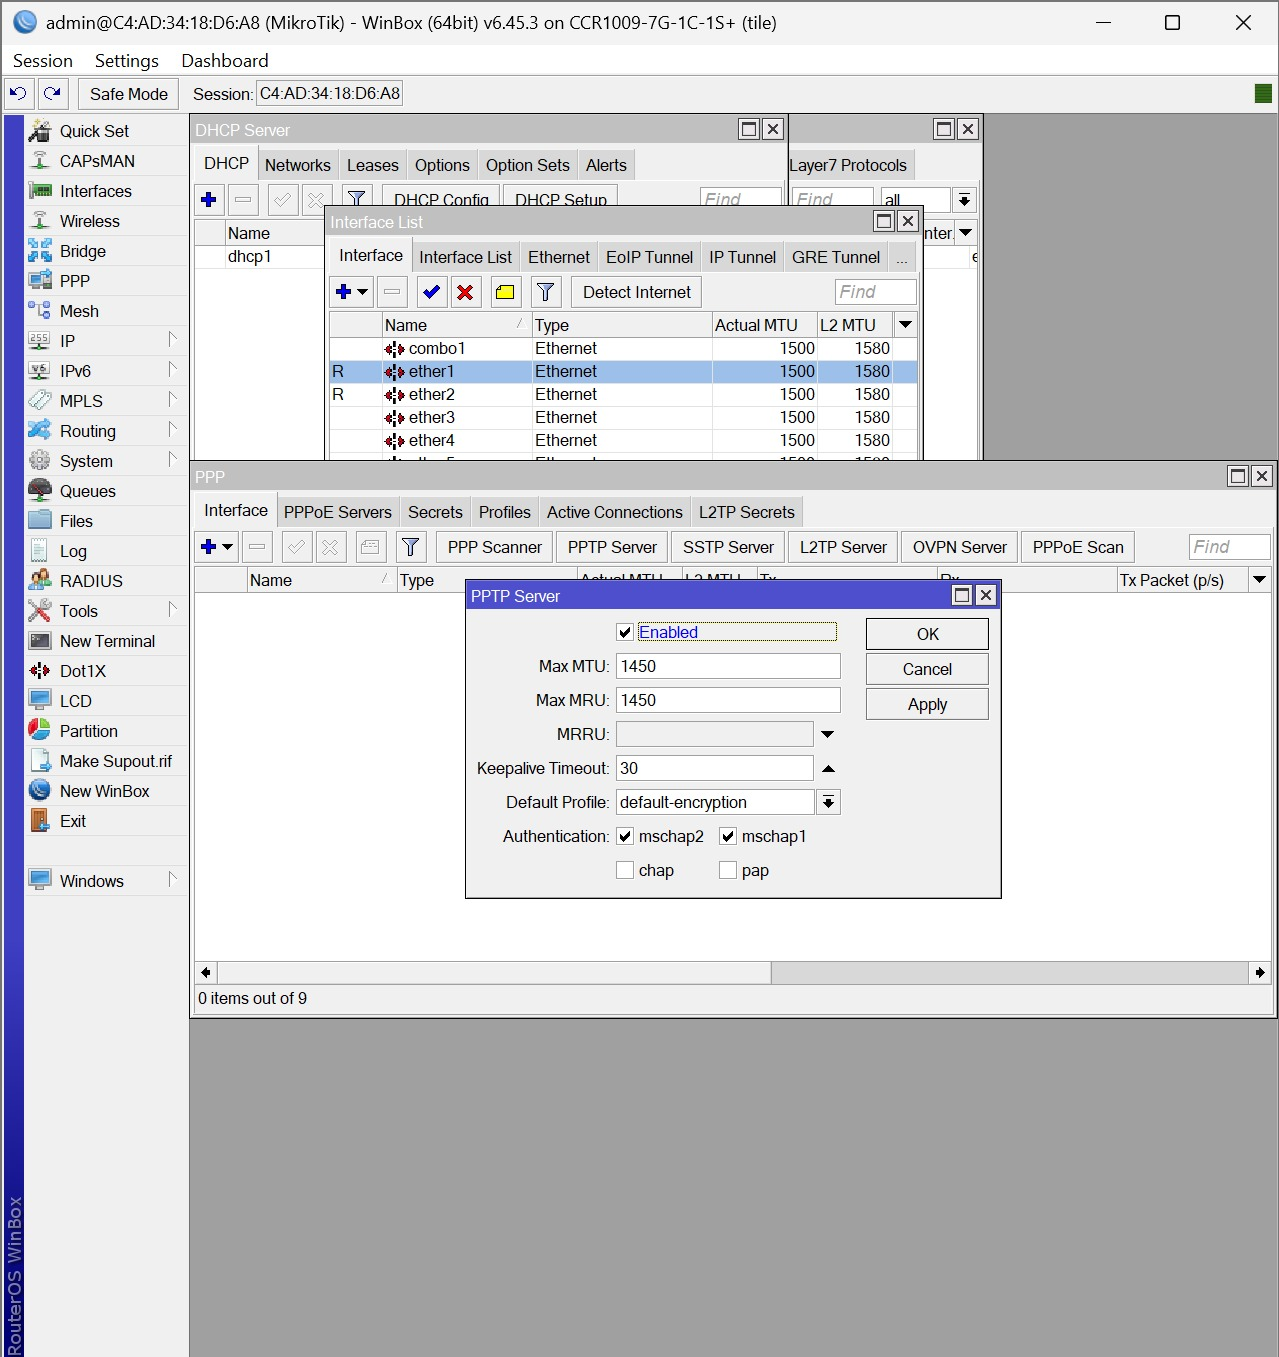
\includegraphics[width=0.5\linewidth]{P1/img/gambar7.jpeg}
        \caption{Konfigurasi PPTP server dilakukan pada router Mikrotik}
        \label{fig:PPTP-server-mikrotik}
    \end{figure}
    
    \item Menyiapkan user dan sandi untuk autentikasi
    \begin{figure}[H]
        \centering
        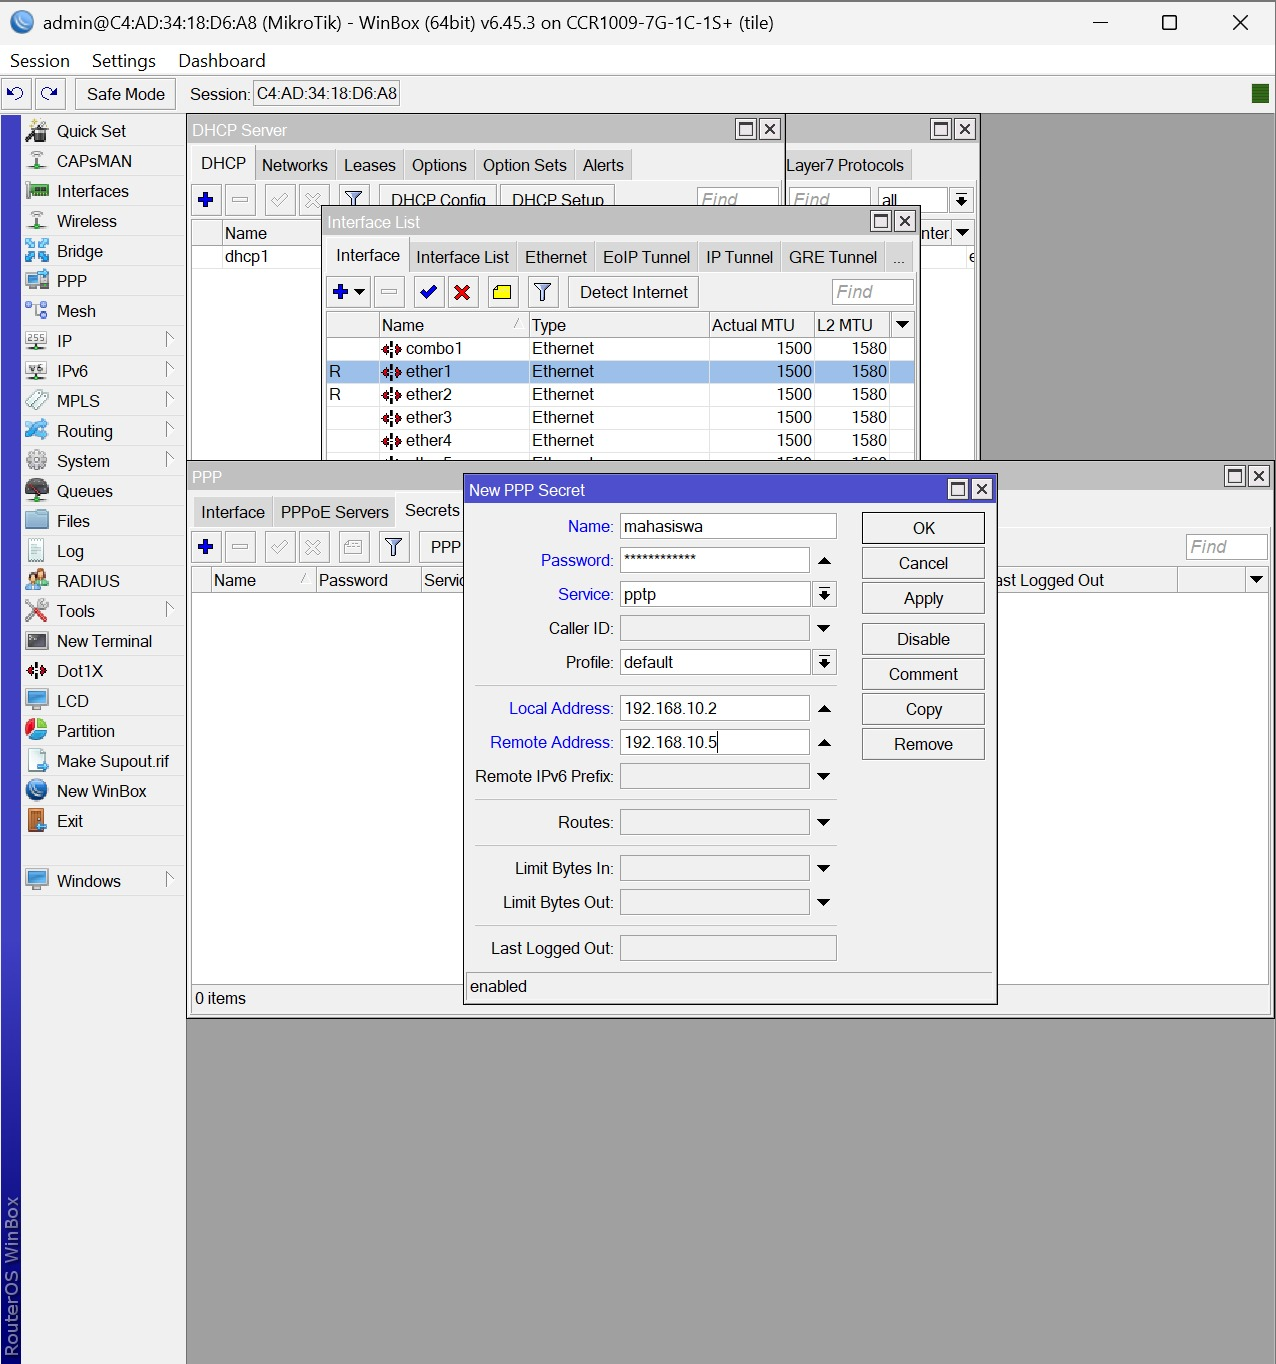
\includegraphics[width=0.5\linewidth]{P1/img/gambar8.jpeg}
        \caption{Konfigurasi user dan password dilakukan pada Mikrotik}
        \label{fig:User-password-mikrotik}
    \end{figure}
    
    \item PPTP client dikonfigurasi di perangkat laptop
    \begin{figure}[H]
        \centering
        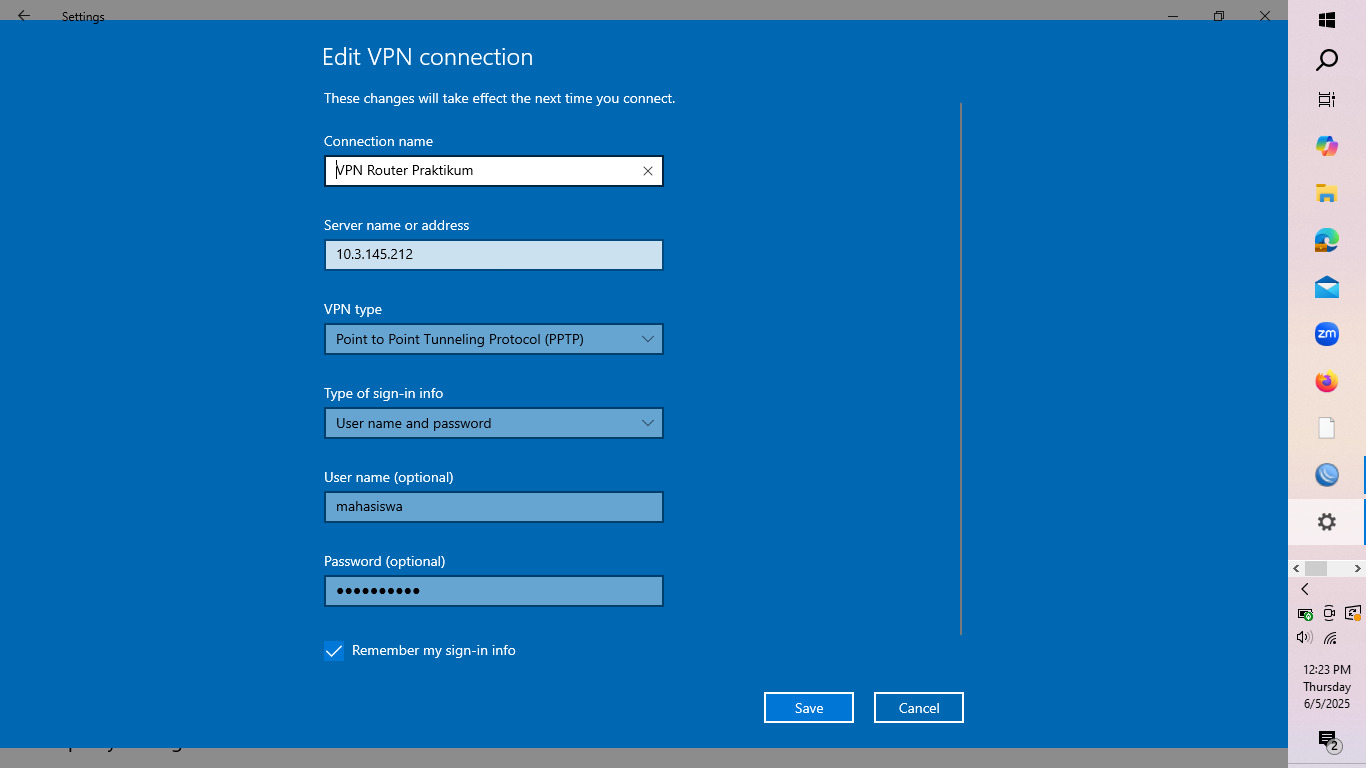
\includegraphics[width=0.5\linewidth]{P1/img/gambar9.jpeg}
        \caption{Melakukan konfigurasi klien PPTP di laptop}
        \label{fig:PPTP-client-laptop}
    \end{figure}
    
    \item Melakukan pengecekan konektivitas 
    \begin{figure}[H]
        \centering
        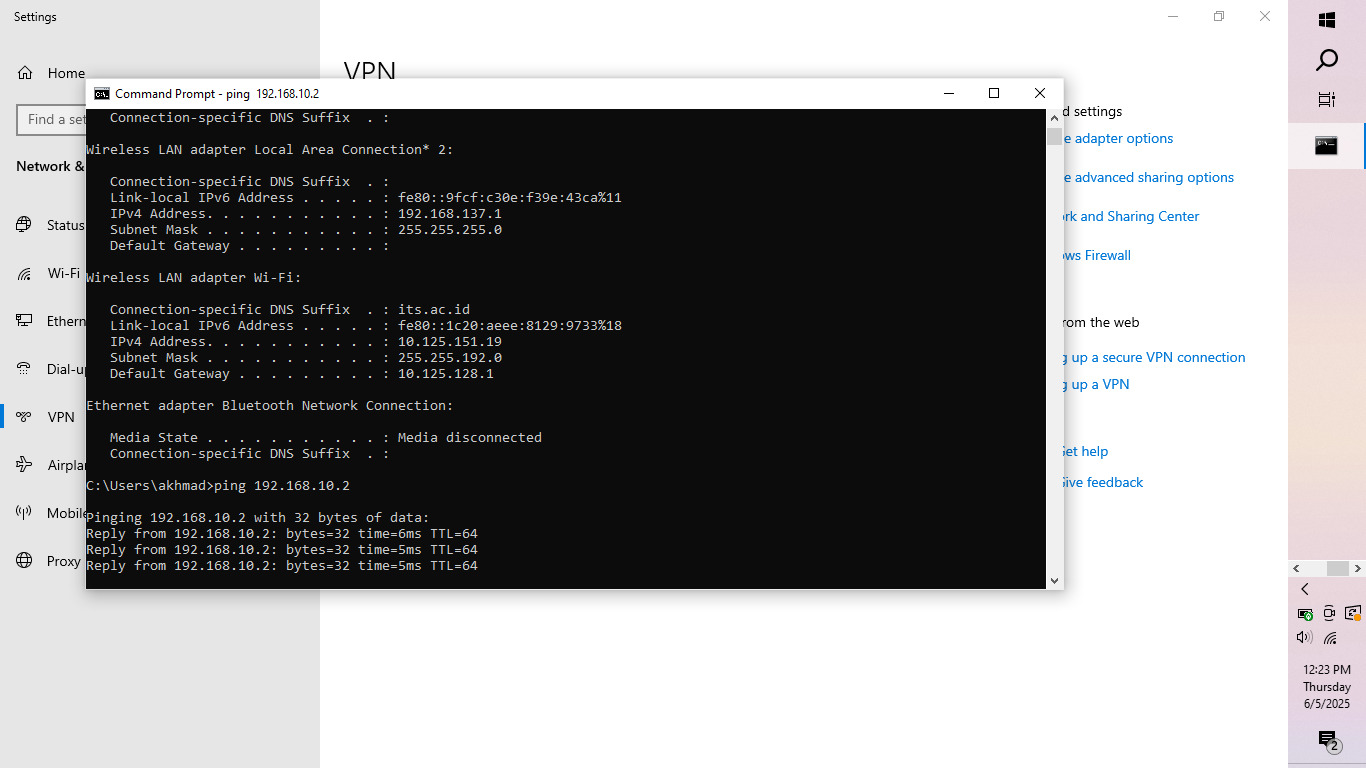
\includegraphics[width=0.5\linewidth]{P1/img/gambar10.jpeg}
        \caption{Verifikasi konektivitas klien PPTP di laptop}
        \label{fig:Verifikasi-koneksi-laptop}
    \end{figure}

    \begin{figure}[H]
        \centering
        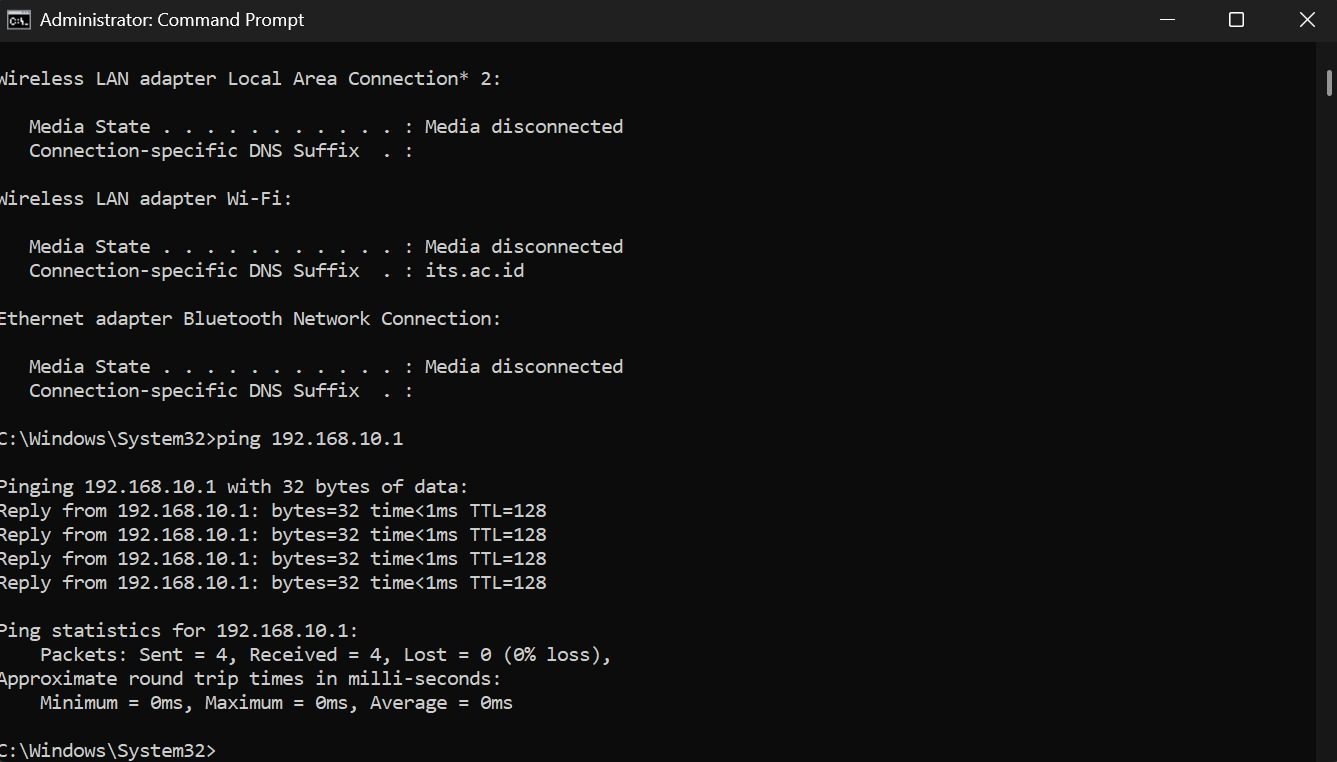
\includegraphics[width=0.5\linewidth]{P1/img/gambar10b.jpeg}
        \caption{Verifikasi konektivitas klien PPTP di laptop}
        \label{fig:Verifikasi-koneksi-laptop}
    \end{figure}


    \item Konfigurasi aturan simple queue untuk kontrol bandwidth
    \begin{figure}[H]
        \centering
        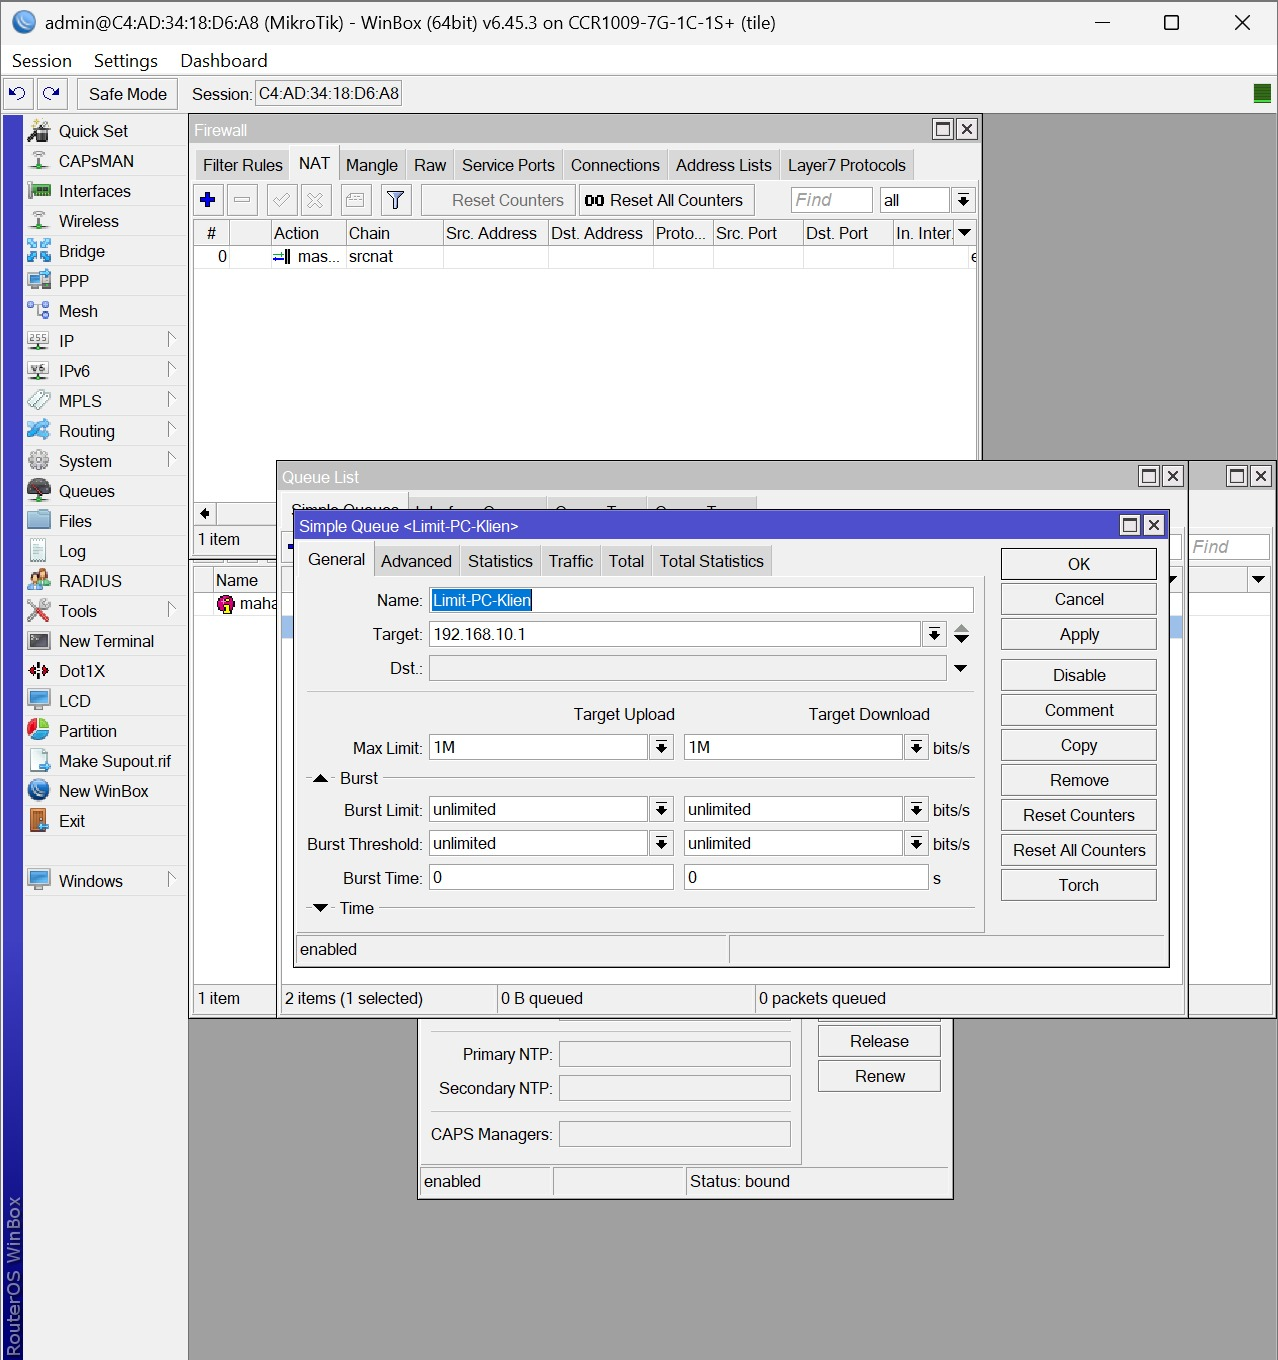
\includegraphics[width=0.5\linewidth]{P1/img/gambar11.jpeg}
        \caption{Konfigurasi simple queue dilakukan di Mikrotik}
        \label{fig:Simple-queue-mikrotik}
    \end{figure}
    
    \item Monitoring traffic yang sedang digunakan
    \begin{figure}[H]
        \centering
        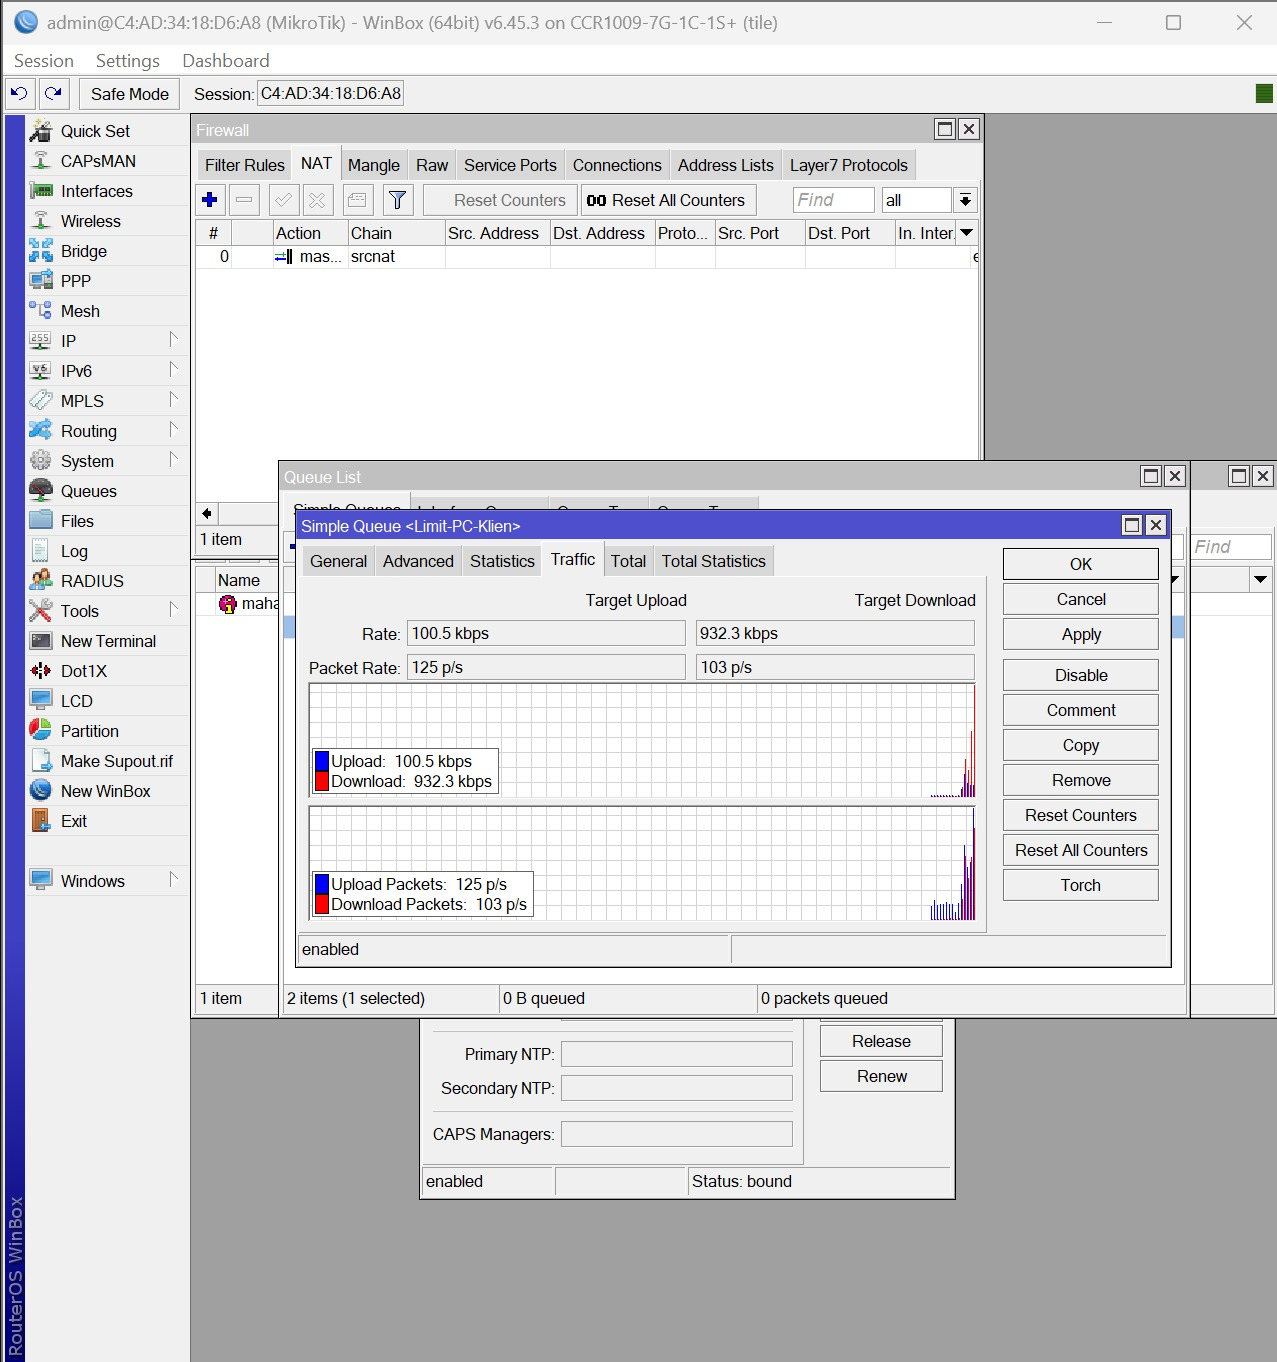
\includegraphics[width=0.5\linewidth]{P1/img/gambar12.jpeg}
        \caption{Mengawasi penggunaan bandwidth di Mikrotik}
        \label{fig:Monitoring-trafik-mikrotik}
    \end{figure}

    \item Menguji koneksi internet menggunakan fitur queue
    \begin{figure}[H]
        \centering
        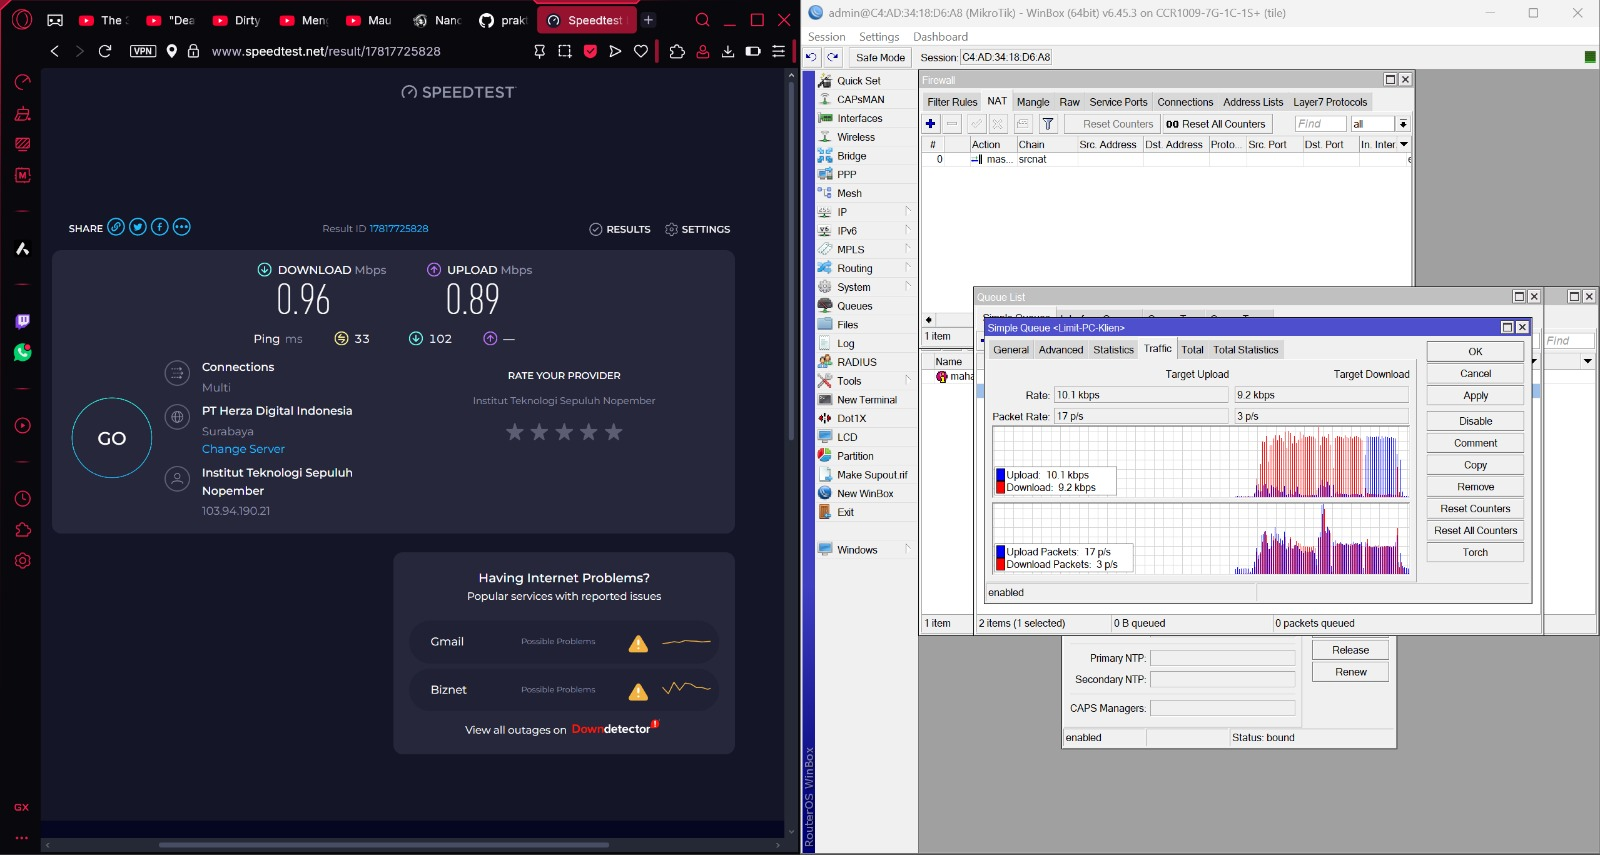
\includegraphics[width=0.5\linewidth]{P1/img/gambar13.jpeg}
        \caption{Verifikasi koneksi internet pada Mikrotik setelah penerapan queue dengan batasan bandwidth}
        \label{fig:Pengujian-koneksi-internet-mikrotik}
    \end{figure}

    \begin{figure}[H]
        \centering
        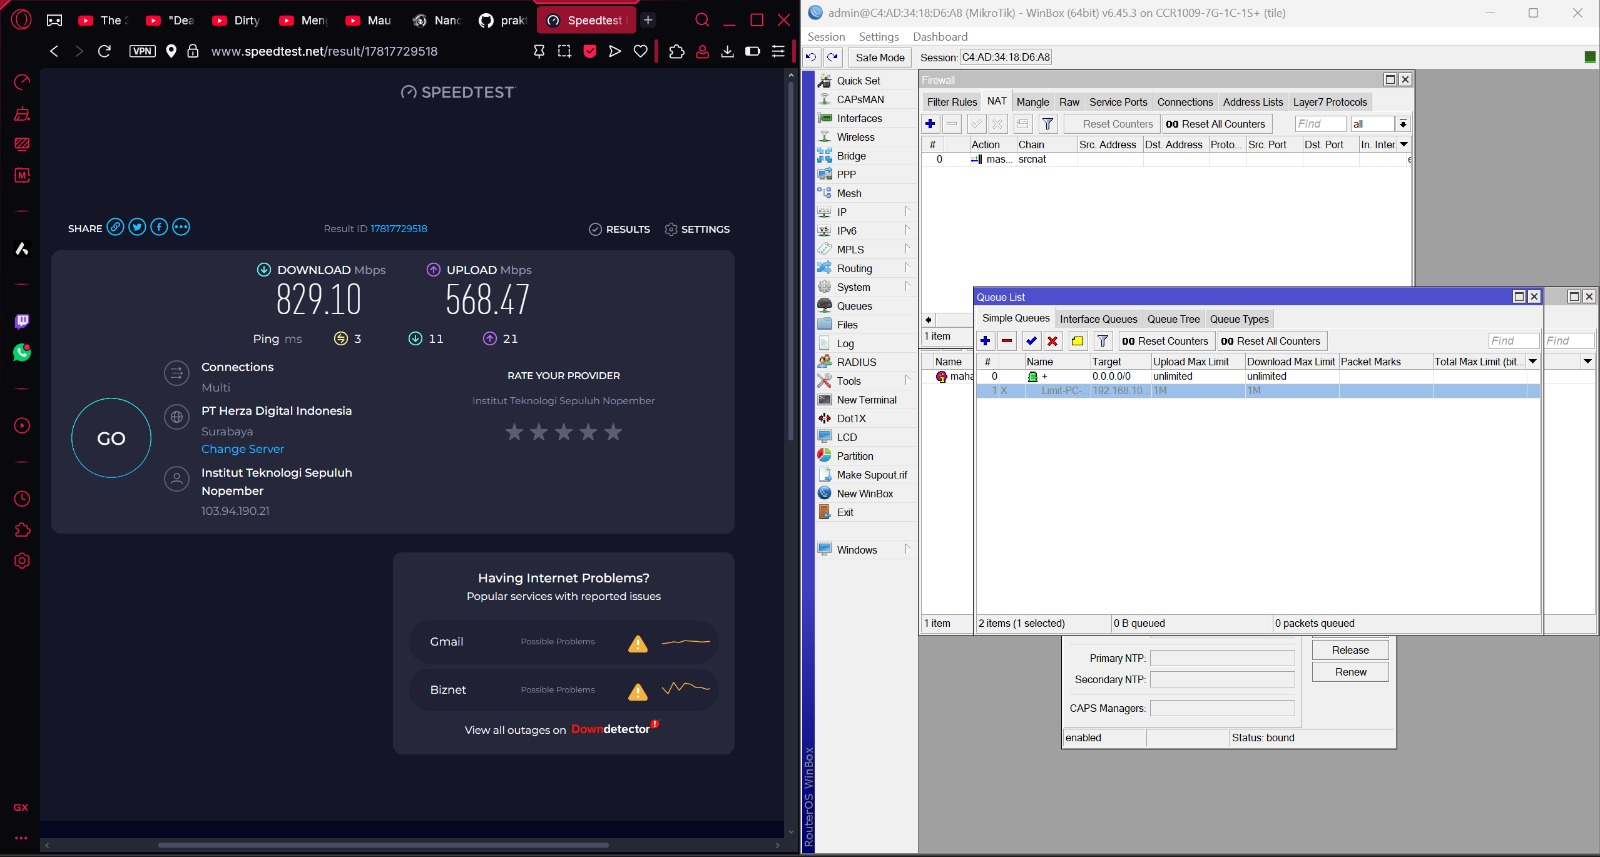
\includegraphics[width=0.5\linewidth]{P1/img/gambar14.jpeg}
        \caption{Verifikasi koneksi internet pada Mikrotik setelah penerapan queue dengan batasan bandwidth}
        \label{fig:Pengujian-koneksi-internet-mikrotik-2}
    \end{figure}

\end{enumerate}


\section{Analisis Hasil Percobaan}

Dalam percobaan ini, konfigurasi Virtual Private Network (VPN) dengan protokol Point-to-Point Tunneling Protocol (PPTP) berhasil diterapkan antara laptop dan router Mikrotik. Proses seperti mengaktifkan server PPTP, membuat akun pengguna beserta kata sandi, hingga menyetel klien PPTP pada laptop, menunjukkan hasil yang memuaskan dengan keberhasilan koneksi antara perangkat klien dan server VPN. Koneksi ini memungkinkan klien untuk terhubung ke jaringan lokal secara aman melalui jalur yang terenkripsi, meskipun berada di jaringan yang berbeda. Fitur ini sangat berguna untuk mengakses jaringan internal dari jarak jauh dengan keamanan data yang terjamin melalui mekanisme tunneling. Selain itu, pengaturan Quality of Service (QoS) menggunakan fitur simple queue juga berhasil dilakukan. Dengan mengatur batas bandwidth tertentu untuk masing-masing pengguna, router Mikrotik mampu mendistribusikan dan mengatur sumber daya jaringan secara optimal. Dari hasil pengujian, terlihat bahwa penggunaan bandwidth oleh klien dapat dibatasi sesuai dengan parameter yang telah ditetapkan, sehingga distribusi jaringan menjadi lebih merata dan terpantau. Fitur pemantauan trafik juga memberikan tampilan visual secara real-time mengenai penggunaan bandwidth, yang sangat membantu dalam mengevaluasi performa jaringan dan mengidentifikasi kemacetan lalu lintas data. Gabungan implementasi VPN dan QoS ini membuktikan bahwa perangkat Mikrotik dapat diandalkan untuk menciptakan jaringan yang aman dan efisien, baik untuk kebutuhan jaringan berskala kecil maupun menengah.

\section{Hasil Tugas Modul}

    \begin{figure}[H]
        \centering
        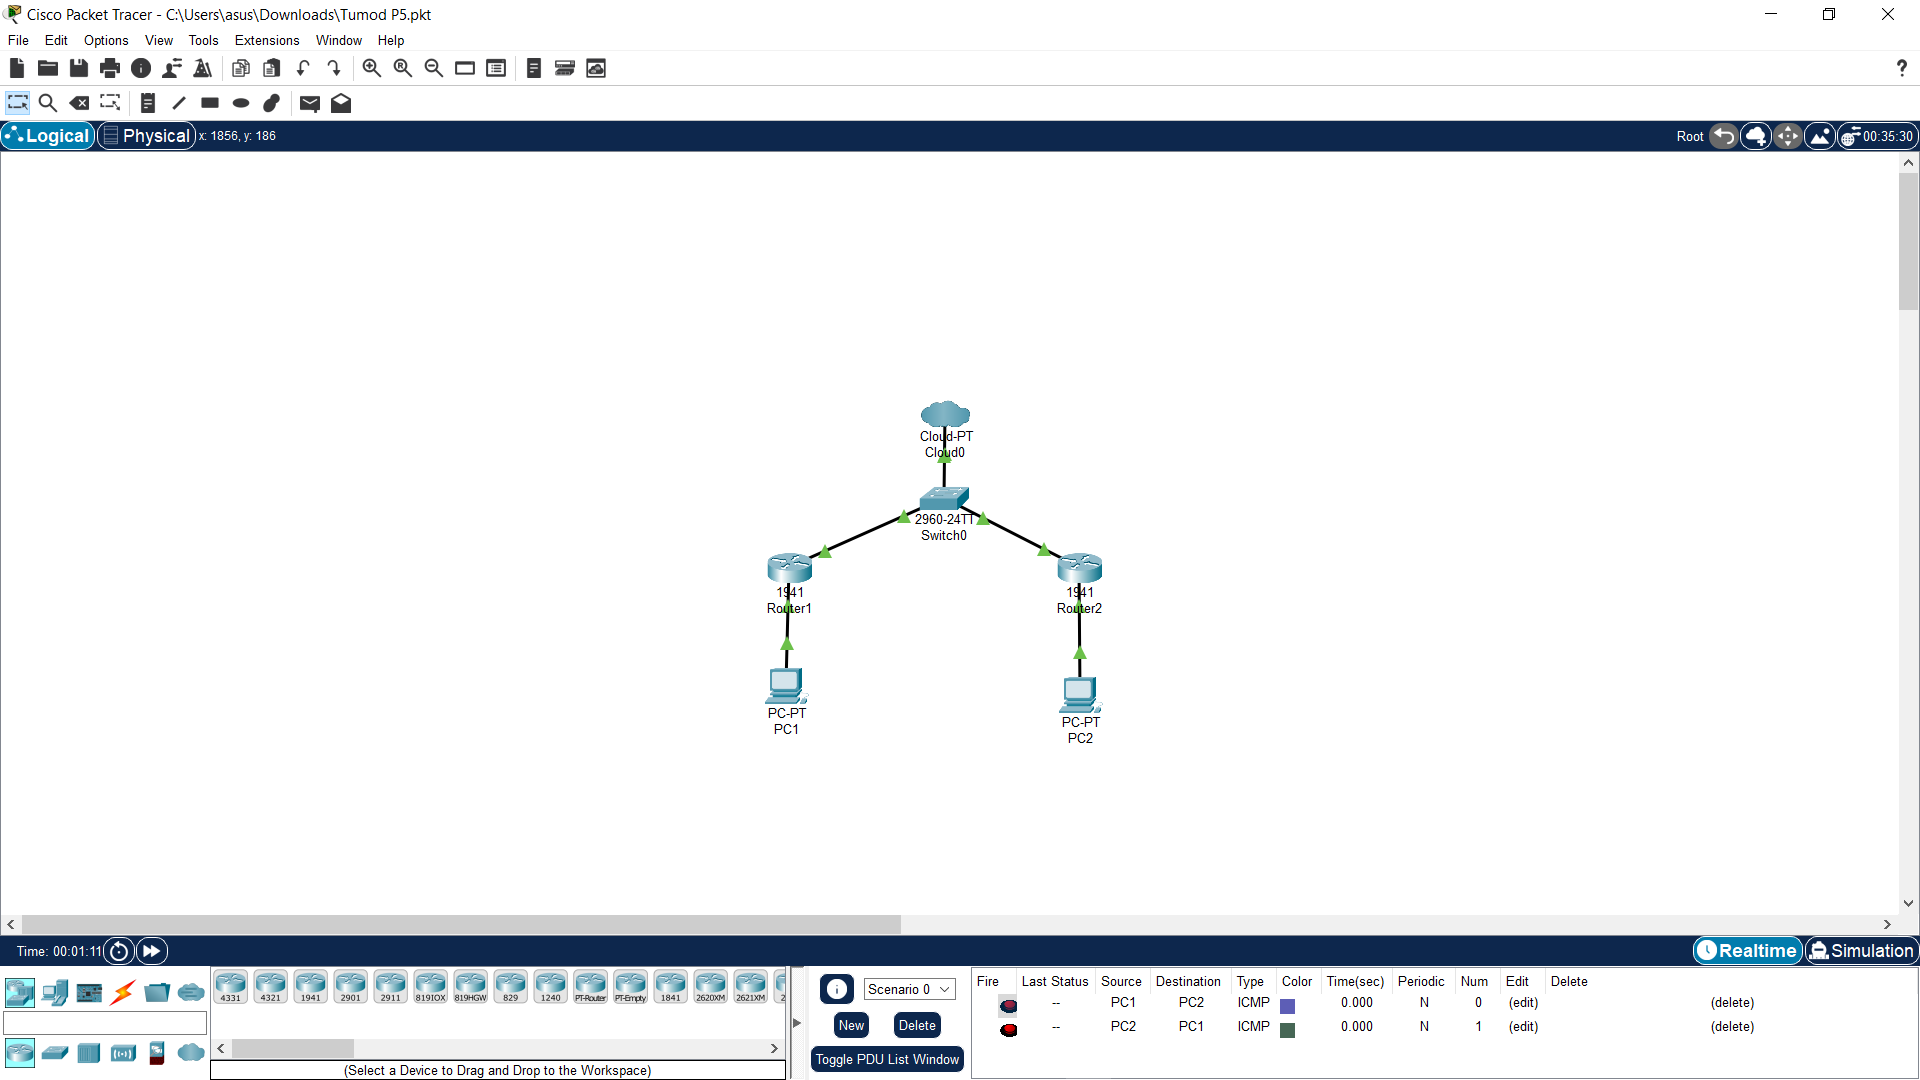
\includegraphics[width=0.5\linewidth]{P1/img/topologi.png}
        \caption{Topologi Jaringan}
        \label{fig:Topologi-jaringan}
    \end{figure}

    \begin{figure}[H]
        \centering
        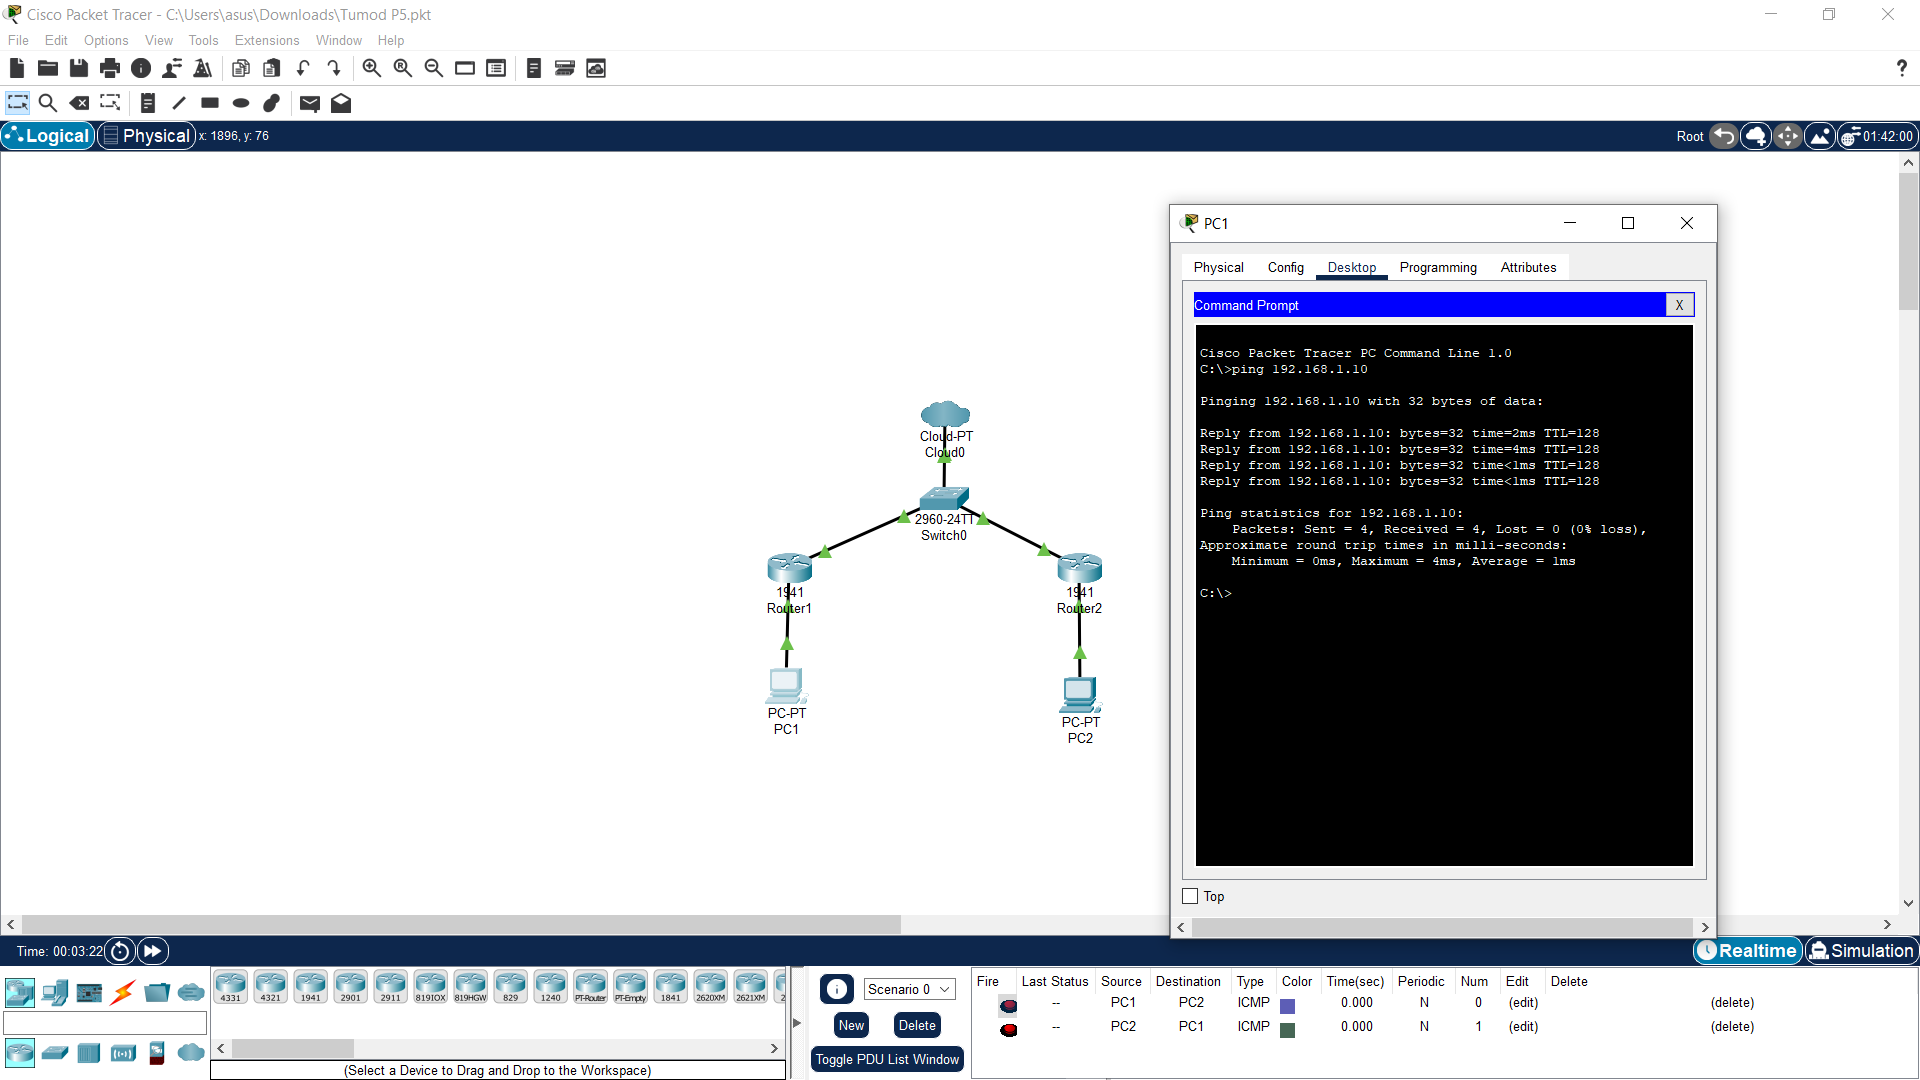
\includegraphics[width=0.5\linewidth]{P1/img/pc1.png}
        \caption{Ping PC 1}
        \label{fig:Pengujian-koneksi}
    \end{figure}

    \begin{figure}[H]
        \centering
        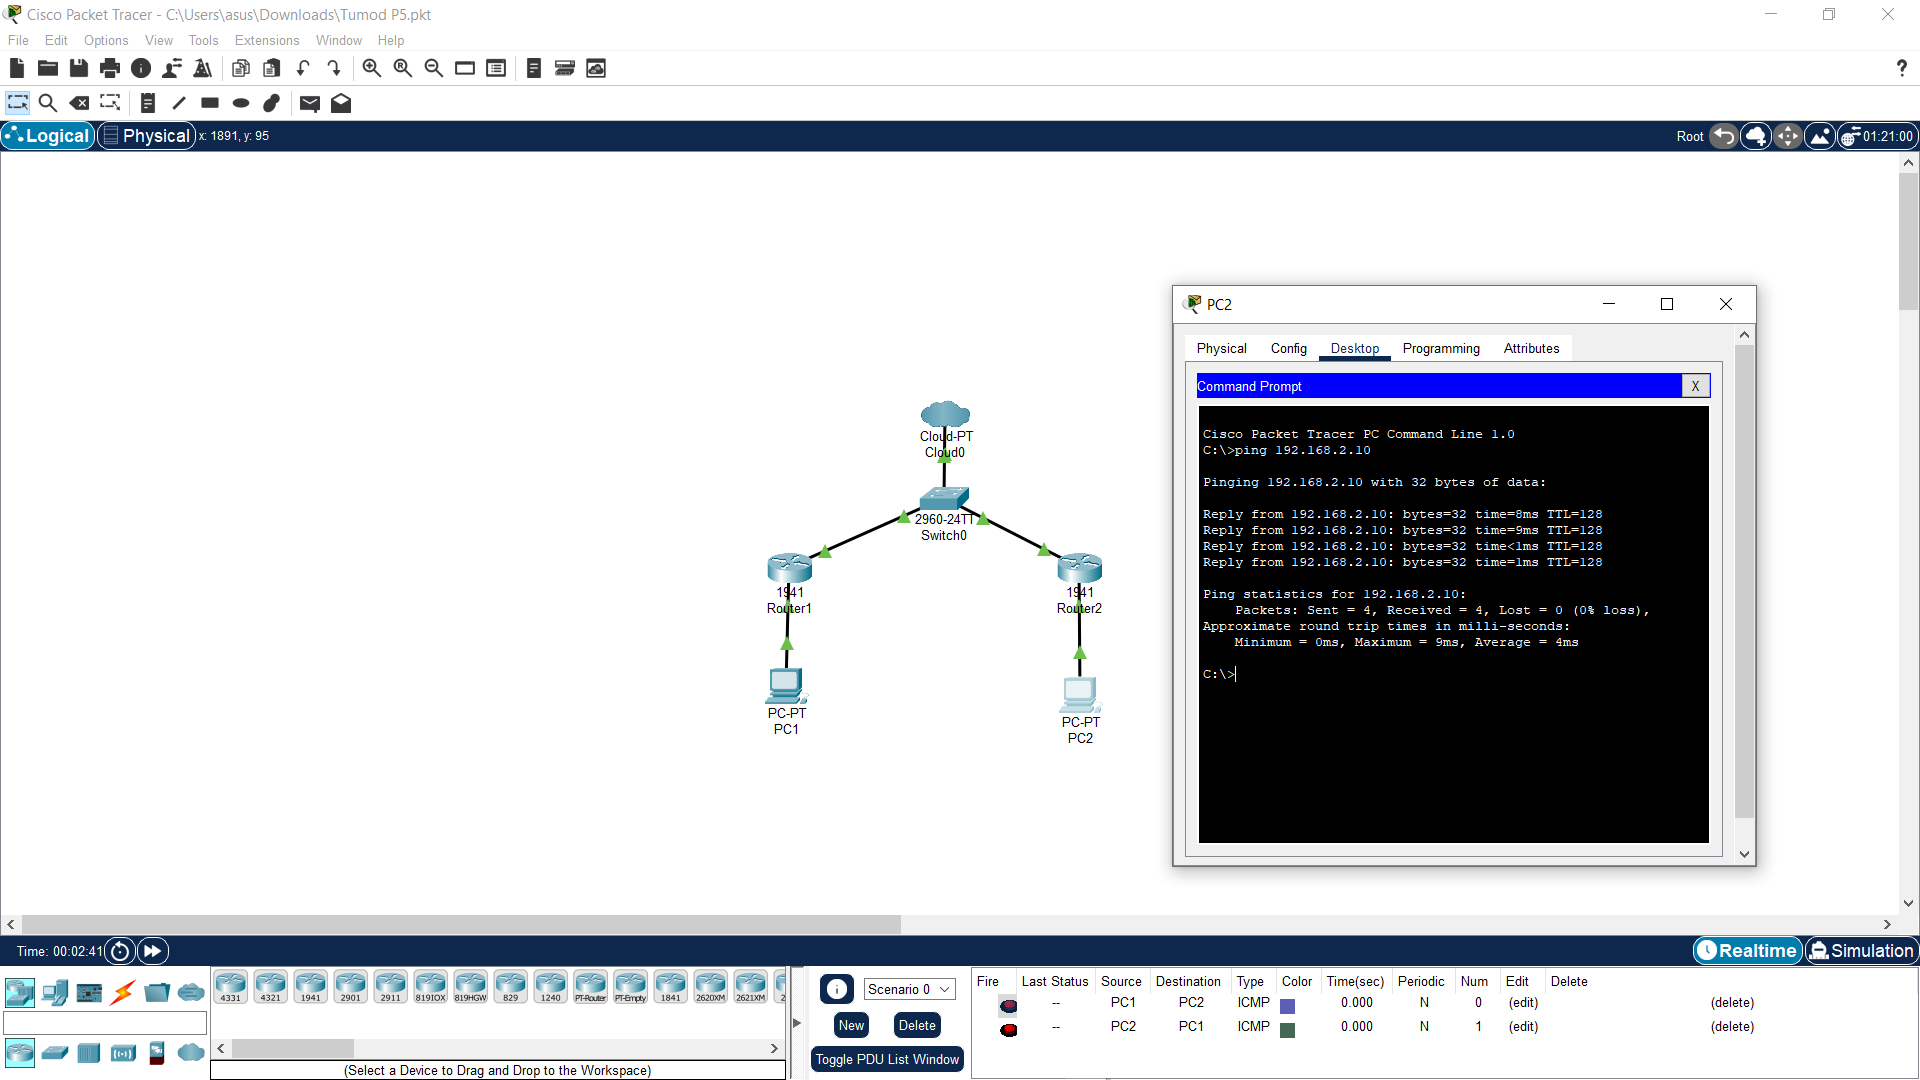
\includegraphics[width=0.5\linewidth]{P1/img/pc2.png}
        \caption{Ping PC 2}
        \label{fig:Pengujian-koneksi}
    \end{figure}

Pada simulasi ini, protokol PPTP membentuk terowongan virtual yang menghubungkan Router 1 dan Router 2 melalui internet. Terowongan ini memungkinkan komunikasi yang aman antara PC1 dan PC2, seolah-olah berada dalam satu jaringan lokal, meskipun data dikirim melalui jaringan publik yang tidak terenkripsi.

\section{Kesimpulan}
Setelah praktikum ini dilaksanakan, dapat disimpulkan bahwa penerapan VPN (Virtual Private Network) dengan protokol PPTP (Point-to-Point Tunneling Protocol) telah berhasil dilakukan. VPN terbukti bermanfaat dalam mengamankan koneksi jaringan serta memungkinkan akses ke jaringan lokal dari lokasi yang jauh. Selain itu, konfigurasi Quality of Service (QoS) menggunakan fitur simple queue pada perangkat Mikrotik juga telah berhasil dijalankan. Fitur ini memungkinkan pembagian bandwidth untuk tiap pengguna, sehingga mendukung pengelolaan lalu lintas jaringan secara lebih efisien dan memastikan pemanfaatan sumber daya jaringan secara maksimal.

\section{Lampiran}
\subsection{Dokumentasi saat praktikum}

    \begin{figure}[H]
        \centering
        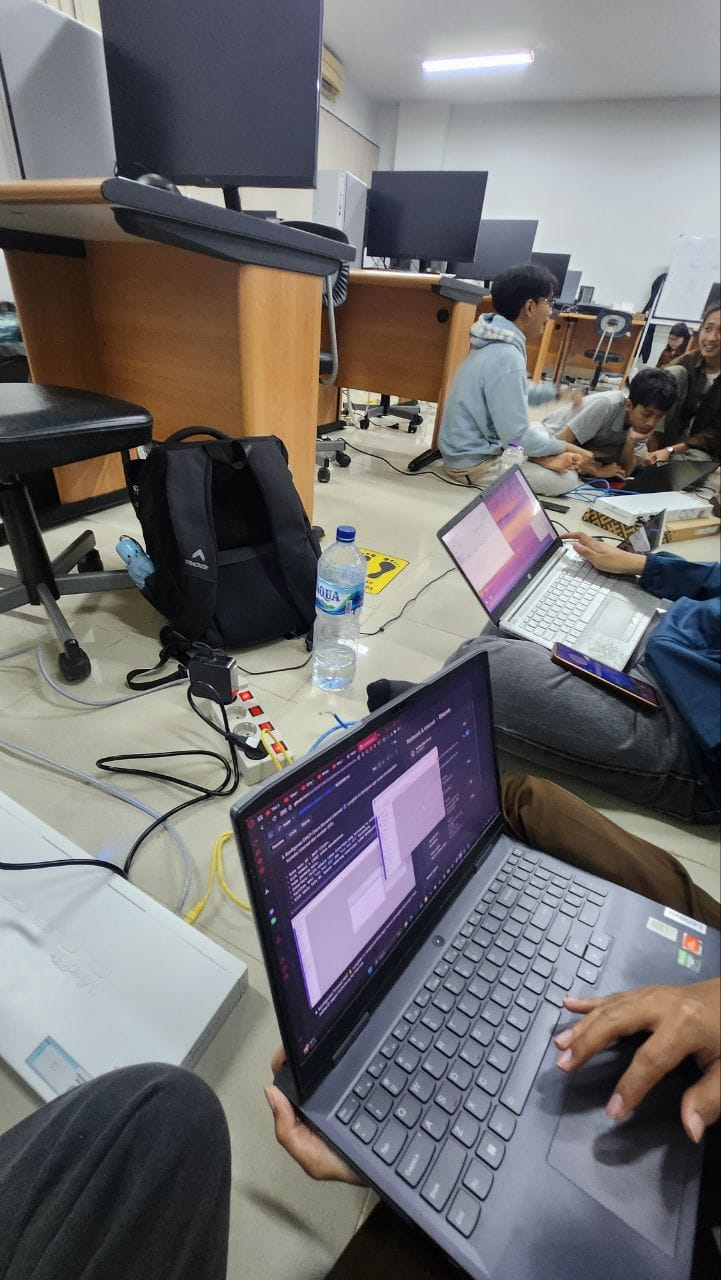
\includegraphics[width=0.5\linewidth]{P1/img/dokum.jpeg}
        \label{fig:Dokum}
    \end{figure}

